\section{Transcript Abundance Estimation}
Before getting a detailed view about \textbf{Transcript Abundance Estimation (TAE)}, we will revisit the \textit{Central Dogma} of genetics: a workflow assumption based on which the whole genetics is based.
\subsection{Central Dogma}
Statement: \textit{\textbf{Instructions on DNA are transcribed onto messenger RNA. Ribosomes are able to read the genetic information inscribed on a strand of messenger RNA and use this information to string amino acids together into a protein.}}~\cite{cdogma2017}.\\
Explanation: The central dogma of molecular biology describes the flow of genetic information in cells from DNA to messenger RNA (mRNA) to protein.  It states that genes specify the sequence of mRNA molecules, which in turn specify the sequence of proteins. In technical terms, the central dogma consists of two steps:\\
\begin{description}
\item [Transcription] The information stored in DNA is so central to cellular function, the cell keeps the DNA protected and copies it in the form of RNA. An enzyme adds one nucleotide to the mRNA strand for every nucleotide it reads in the DNA strand~\cite{cdogma2017}.
\item [Translation]  The translation of information to a protein is more complex because three mRNA nucleotides correspond to one amino acid in the polypeptide sequence~\cite{cdogma2017}.

\begin{figure}[htp]
\centering
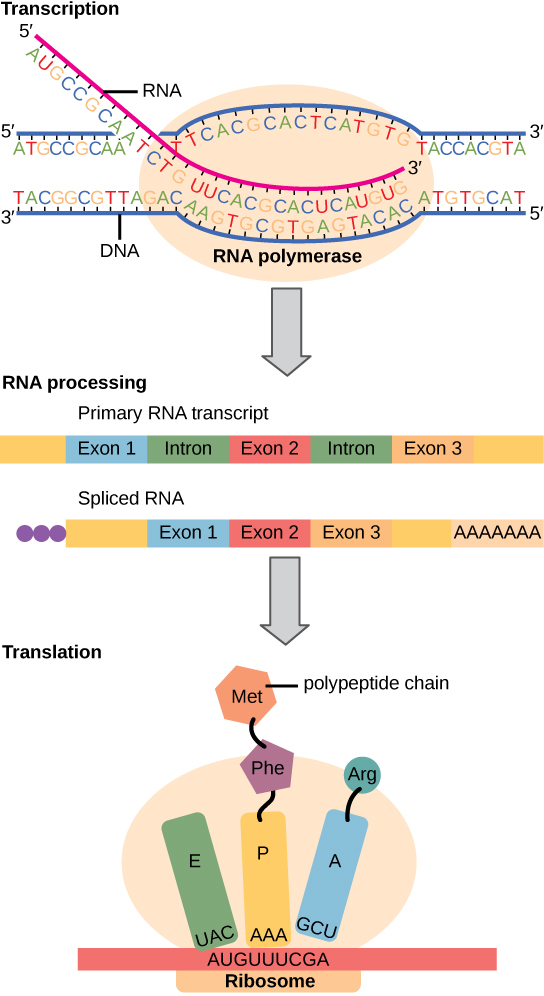
\includegraphics[scale=1.00]{centraldogma.jpeg}
\caption{Central Dogma~\cite{cdogma2017}}
\label{cdog}
\end{figure}
\end{description}

\subsection{Some related terms to know}

\subsubsection{DNA sequencing}
DNA sequencing is the process of determining the precise order of nucleotides within a DNA molecule. It includes any method or technology that is used to determine the order of the four bases—adenine, guanine, cytosine, and thymine—in a strand of DNA~\cite{wiki:dnaseq}. 

\begin{figure}[htp]
\centering
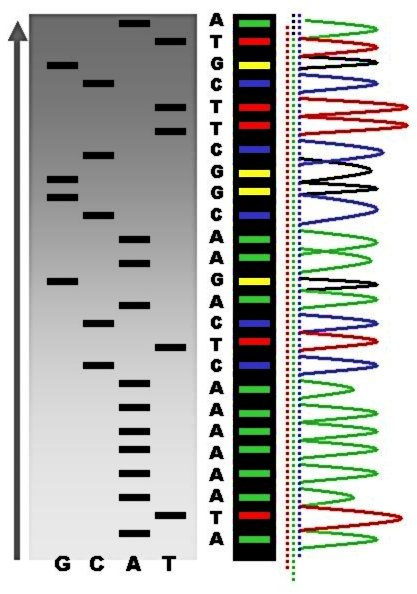
\includegraphics[scale=0.50]{Radioactive_Fluorescent_Seq.jpg}
\caption{An example of the results of automated chain-termination DNA sequencing~\cite{wiki:dnaseq}.}
\label{seq}
\end{figure}
\subsubsection{Transcript}

A primary transcript is the single-stranded ribonucleic acid (RNA) product synthesized by transcription of DNA, and processed to yield various mature RNA products such as mRNAs, tRNAs, and rRNAs. The primary transcripts designated to be mRNAs are modified in preparation for translation. For example, a precursor messenger RNA (pre-mRNA) is a type of primary transcript that becomes a messenger RNA (mRNA) after processing~\cite{wiki:pritrans}.

\subsubsection{Alternative Splicing}
Alternative splicing, or differential splicing, is a regulated process during gene expression that results in a single gene coding for multiple proteins. In this process, particular exons of a gene may be included within or excluded from the final, processed messenger RNA (mRNA) produced from that gene~\cite{ wiki:altsp} (see fig~\ref{iso}).

\subsubsection{Protein Isoform}

A protein isoform, or "protein variant"[1] is a member of a set of highly similar proteins that perform the same or similar biological roles. A set of protein isoforms may be formed from alternative splicings or other post-translational modifications of a single gene~\cite{wiki:proiso} (see figure~\ref{iso}). \begin{figure}[htp]
\centering
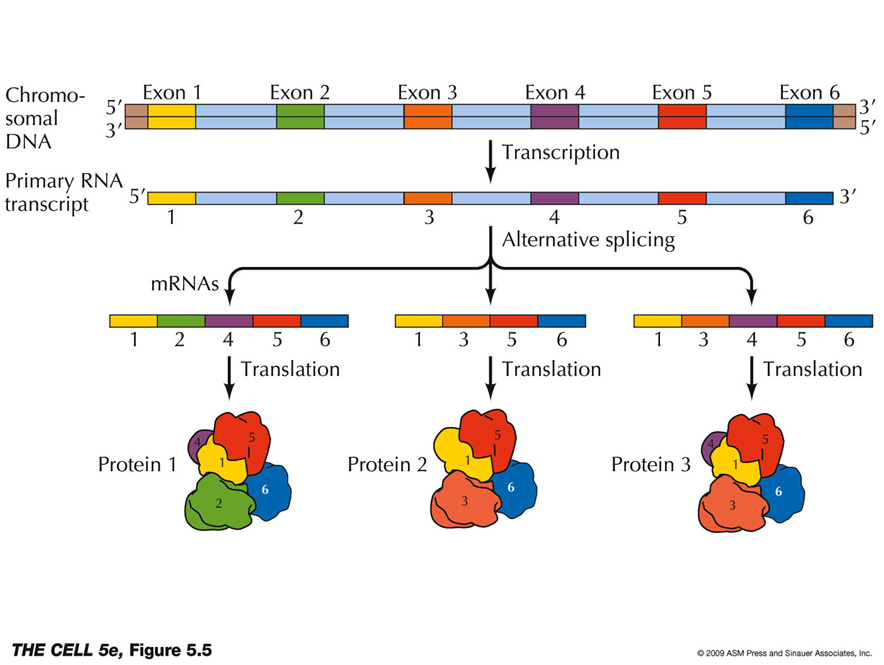
\includegraphics[scale=0.50]{proiso.png}
\caption{Protein A, B and C are isoforms encoded from the same gene through alternative splicing~\cite{wiki:altsp}}
\label{iso}
\end{figure}
\subsubsection{Short Read Alignment}

Short read alignment is the process of figuring out where in the genome a sequence is from. By transcription process we get the mRNAs from DNA. By putting them through a reverse transcription and sequencing pipeline, we can get the sequences corresponding to the RNA transcript. A huge task after this is finding the place in the genome from where that gene sequence generated. This is done by short read alignment algorithms.

\subsubsection{*-seq}
*-seq is a generalized term used to denote the class of high-throughput selection algorithms. The full list of *-seq algorithms can be found at \url{https://liorpachter.wordpress.com/seq/}.

\subsubsection{RNA-seq}
RNA-Seq (RNA sequencing), also called whole transcriptome shotgun sequencing  (WTSS), uses next-generation sequencing (NGS) to reveal the presence and quantity of RNA in a biological sample at a given moment in time. The process of RNA-seq has been described in~\cite{wiki:rnaseq} (see figure~\ref{rnaseq}.

\begin{figure}[htp]
\centering
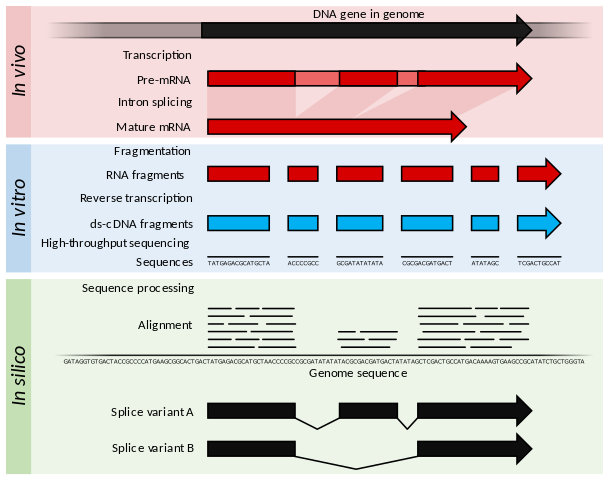
\includegraphics[scale=0.70]{Summary_of_RNA-Seq.svg.png}
\caption{Summary of RNA-Seq. Within the organisms, genes are transcribed and spliced (in eukaryotes) to produce mature mRNA transcripts (red). The mRNA is extracted from the organism, fragmented and copied into stable ds-cDNA(blue). The ds-cDNA is sequenced using high-throughput, short-read sequencing methods. These sequences can then be aligned to a reference genome sequence to reconstruct which genome regions were being transcribed. This data can be used to annotate where expressed genes are, their relative expression levels, and any alternative splice variants~\cite{wiki:rnaseq}.}
\label{rnaseq}
\end{figure} 

\subsection{Relative Transcript Abundance Estimation}

Sequencing RNAs are easier than sequencing proteins. In genetics, there might often be the necessity of knowing the proportion of proteins present in a cell. However, as protein sequencing is replaced by RNA-sequencing as a proxy, we are interested in finding the \textit{Relative Transcript Abundance} of the RNA-transcripts: which deals with the percentage amount of the RNA-transcripts present in a set of cell or genome reads.\\ 

\subsubsection{Challenges and motivation}
Usually, in theoritical term, to compute the relative abundances, it is obvious to count the amount of reads from a transcript and deduce the parameters thereby. But there are some challenges. Due to the presence of isoform, it can happen that a single sequence read may be mapped to multiple transcripts while short read mapping. This multiple mapping pushes us to use the expected number of reads from each transcripts rather than using their exact numbers (remember using the expected number of heads and tails from coins A \& B instead of using the exact counts because we did not know which coins were tossed?).\\
But to use expected value, we need to know the relative abundance of the transcripts again. This poses a deadlock like situation as the coin bias problem stated in previous section, where to know the biases of the coins, we needed to know the expected numbers of heads and tails from different coins, which in turn needed to use coin biases. We solved that problem using EM algorithm. This abundance estimation problem won't be the exception too.\\


In the next section, we will discuss a mathematical model of relative abundance estimation and try to solve it using EM algorithm.